\documentclass[aspectratio=169]{beamer}
\usetheme{Madrid}
\usecolortheme{default}

% Packages
\usepackage{graphicx}
\usepackage{booktabs}
\usepackage{tikz}
\usepackage{multicol}
\usepackage{amsmath}
\usepackage{xcolor}

% Custom colors (inspired by your example slides)
\definecolor{lightblue}{RGB}{173,216,230}
\definecolor{darkblue}{RGB}{25,25,112}
\definecolor{uwgold}{RGB}{255,197,0}
\definecolor{uwblack}{RGB}{0,0,0}
\definecolor{accentblue}{RGB}{135,206,250}

% Remove navigation symbols and footline
\setbeamertemplate{navigation symbols}{}
\setbeamertemplate{footline}{}

% Theme customization
\setbeamercolor{structure}{fg=darkblue}
\setbeamercolor{title}{fg=darkblue}
\setbeamercolor{frametitle}{fg=darkblue}
\setbeamercolor{block title}{fg=white,bg=lightblue}
\setbeamercolor{block body}{fg=black,bg=lightblue!20}

% Title page information
\title{Omni-Directional Chair for Wheelchair Sports}
\subtitle{Preliminary Design Presentation}
\author{Samuel \and Ameen \and Joseph \and Chanuth \and Adesh}
\institute{MTE 481 - Mechatronics Engineering Design Project\\Capstone Group 52}
\date{October 20, 2025}

\begin{document}

%% TITLE SLIDE
\begin{frame}
\titlepage
\end{frame}

%% AGENDA
\begin{frame}{Presentation Agenda}
\Large
\begin{enumerate}
    \item Problem \& Need Identification
    \item Design Objectives \& Specifications
    \item Alternate Design Concepts
    \item Patent Landscape Review
    \item Technical Details \& Components
    \item Project Timeline
\end{enumerate}
\end{frame}

%% SECTION 1: PROBLEM & NEED
\section{Problem \& Need Identification}

\begin{frame}{The Challenge: Dual Hand Requirement}
\begin{center}
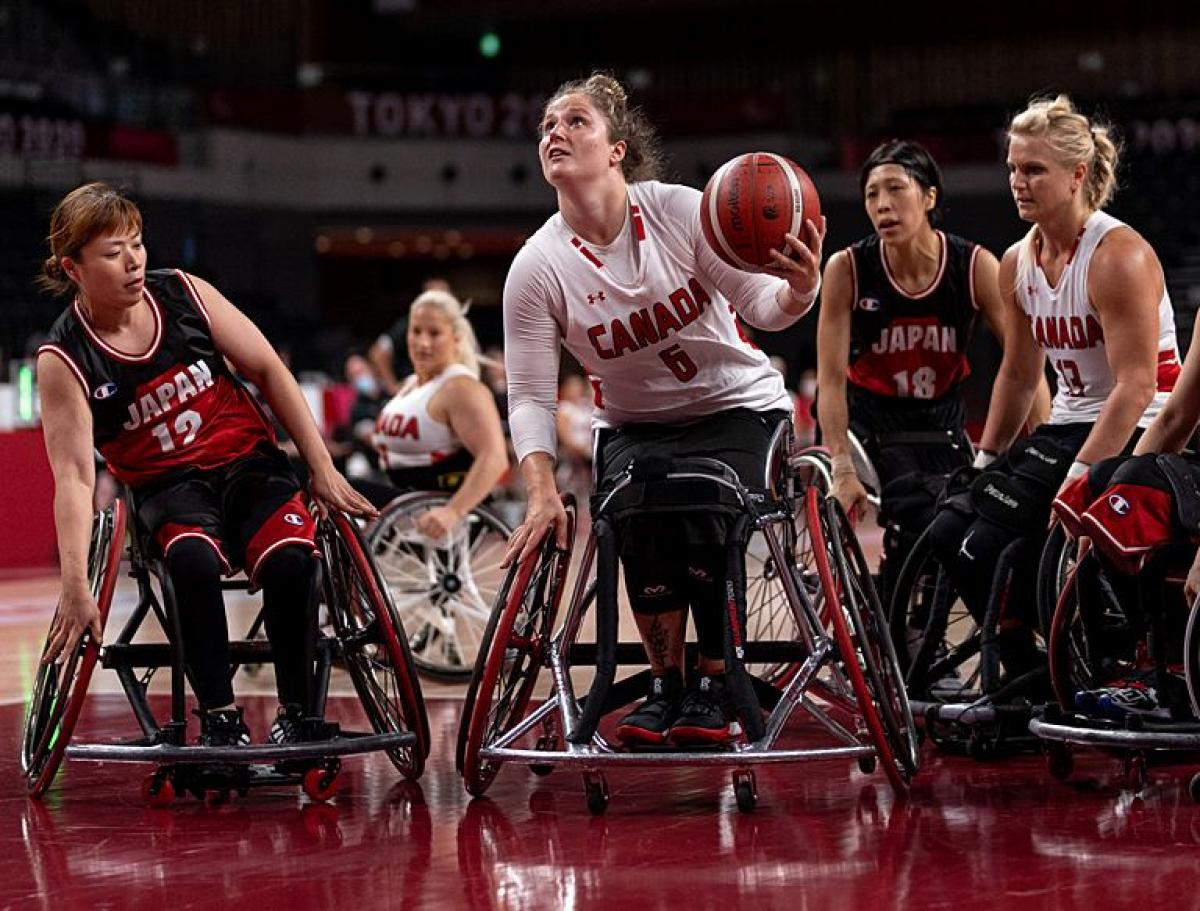
\includegraphics[height=0.5\textheight]{pdpAssets/WheelchairBasketballPlayerPhoto.jpg}
\end{center}

\begin{block}{The Problem}
Wheelchair sports players need BOTH hands for:
\begin{itemize}
    \item \textbf{Wheelchair propulsion} - pushing wheels to move and steer
    \item \textbf{Equipment handling} - dribbling, passing, shooting, racquet sports
\end{itemize}
\end{block}
\end{frame}

\begin{frame}{Impact \& Significance}
\begin{columns}[T]
\begin{column}{0.48\textwidth}
\begin{block}{By the Numbers}
\begin{itemize}
    \item \textcolor{red}{\textbf{73\%}} shoulder pain
    \item \textcolor{red}{\textbf{60-80\%}} arm fatigue
    \item \textcolor{red}{\textbf{15-20}} interruptions/game
    \item \textcolor{red}{\textbf{30-40\%}} lower scoring
\end{itemize}
\end{block}

\vspace{0.4cm}
\begin{block}{User Story}
\textit{"I have to stop dribbling just to reposition my chair — which interrupts gameplay and reduces my reaction speed."}

\vspace{0.3cm}
- Adrit Batra\\
Laurier University
\end{block}
\end{column}

\begin{column}{0.48\textwidth}
\begin{block}{Sports Impact}
Tennis, badminton, hockey currently limited for wheelchair users
\end{block}

\vspace{0.4cm}
\begin{block}{Research Data}
\begin{itemize}
    \item \textbf{Biomechanical Impact}: 73\% injury rate
    \item \textbf{Performance Gap}: 30-40\% lower scoring
    \item \textbf{Accessibility}: 25-40\% participation increase potential
\end{itemize}
\end{block}
\end{column}
\end{columns}
\end{frame}

\begin{frame}{Our Mission}
\begin{columns}[T]
\begin{column}{0.6\textwidth}
\vspace{-0.3cm}
\begin{block}{The Vision}
\Large \textbf{Revolutionize wheelchair sports} through hands-free mobility technology
\end{block}

\vspace{-0.2cm}
\begin{block}{Core Innovation}
\begin{itemize}
    \item \textbf{Body-shift control} - natural, intuitive movement
    \item \textbf{Sports-optimized} - designed for competitive play
    \item \textbf{Equipment-friendly} - no interference with gear
\end{itemize}
\end{block}

\vspace{-0.2cm}
\begin{block}{Target Impact}
\begin{itemize}
    \item \textbf{25-40\%} increase in sports participation
    \item \textbf{73\%} reduction in shoulder injuries
    \item \textbf{New sports access} - tennis, badminton, hockey
    \item \textbf{Enhanced performance} - competitive advantage
\end{itemize}
\end{block}
\end{column}

\begin{column}{0.38\textwidth}
\begin{center}
\Large \textbf{Breaking Barriers}

\vspace{0.3cm}
\normalsize
\textit{"I have to stop dribbling just to reposition my chair — which interrupts gameplay and reduces my reaction speed."}

\vspace{0.3cm}
- Adrit Batra\\
Laurier University

\vspace{0.2cm}
\begin{block}{The Solution}
Hands-free wheelchair that responds to body weight shifts, enabling simultaneous movement and equipment handling
\end{block}
\end{center}
\end{column}
\end{columns}
\end{frame}

%% SECTION 2: DESIGN OBJECTIVES
\section{Design Objectives}

\begin{frame}{Key Engineering Specifications}
\begin{columns}[T]
\begin{column}{0.48\textwidth}
\begin{block}{Performance}
\begin{itemize}
    \item Speed: \textbf{5 mph}
    \item Response: \textbf{<100ms}
    \item Movement: \textbf{3 DOF}
    \item Battery: \textbf{2+ hours}
\end{itemize}
\end{block}

\begin{block}{Control}
\begin{itemize}
    \item Method: Body-shift
    \item 100\% hands-free
    \item Intuitive operation
\end{itemize}
\end{block}
\end{column}

\begin{column}{0.48\textwidth}
\begin{block}{Safety \& Physical}
\begin{itemize}
    \item Collision: \textbf{40N resistance}
    \item Load: \textbf{200 lbs}
    \item Emergency stop
    \item Stability factor: $>1.5$
\end{itemize}
\end{block}

\begin{block}{Constraints}
\begin{itemize}
    \item Budget: \textbf{$<\$300$}
    \item Timeline: \textbf{May 2026}
    \item Environmental: 5\% contamination
\end{itemize}
\end{block}
\end{column}
\end{columns}
\end{frame}

\begin{frame}{Design Constraints}
\begin{block}{Critical Requirements}
\begin{itemize}
    \item \textbf{C1:} Hands-Free Control - 100\% movement without hand input
    \item \textbf{C2:} Safety - Withstand 30-50N collision forces
    \item \textbf{C3:} Equipment Compatibility - No interference with sports gear
    \item \textbf{C4:} Environmental - Handle 5\% surface contamination
    \item \textbf{C5:} Response Time - $<100$ms system lag
    \item \textbf{C6:} Budget - $<\$300$ total project cost
    \item \textbf{C7:} Timeline - Prototype by May 2026 symposium
\end{itemize}
\end{block}
\end{frame}

%% SECTION 3: ALTERNATE DESIGNS
\section{Alternate Designs}

\begin{frame}{Four Design Concepts Evaluated}
\begin{center}
\begin{tabular}{cc}
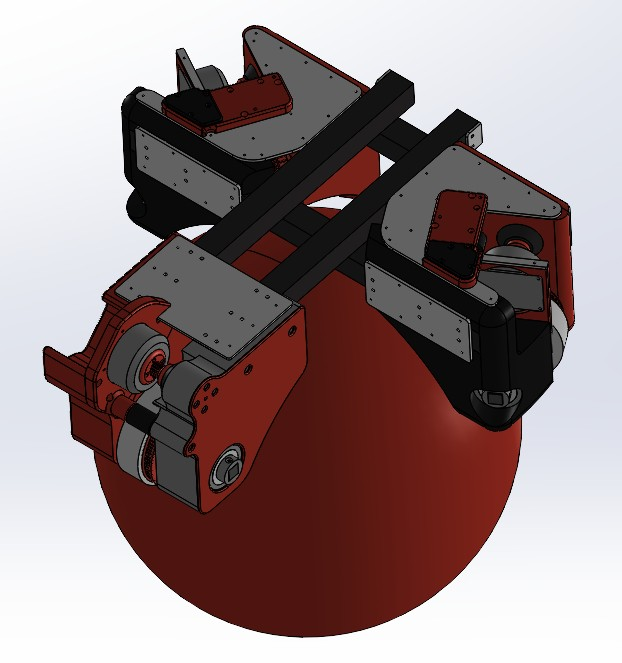
\includegraphics[height=0.25\textheight]{pdpAssets/PreliminaryDesignCadRendering.jpg} &
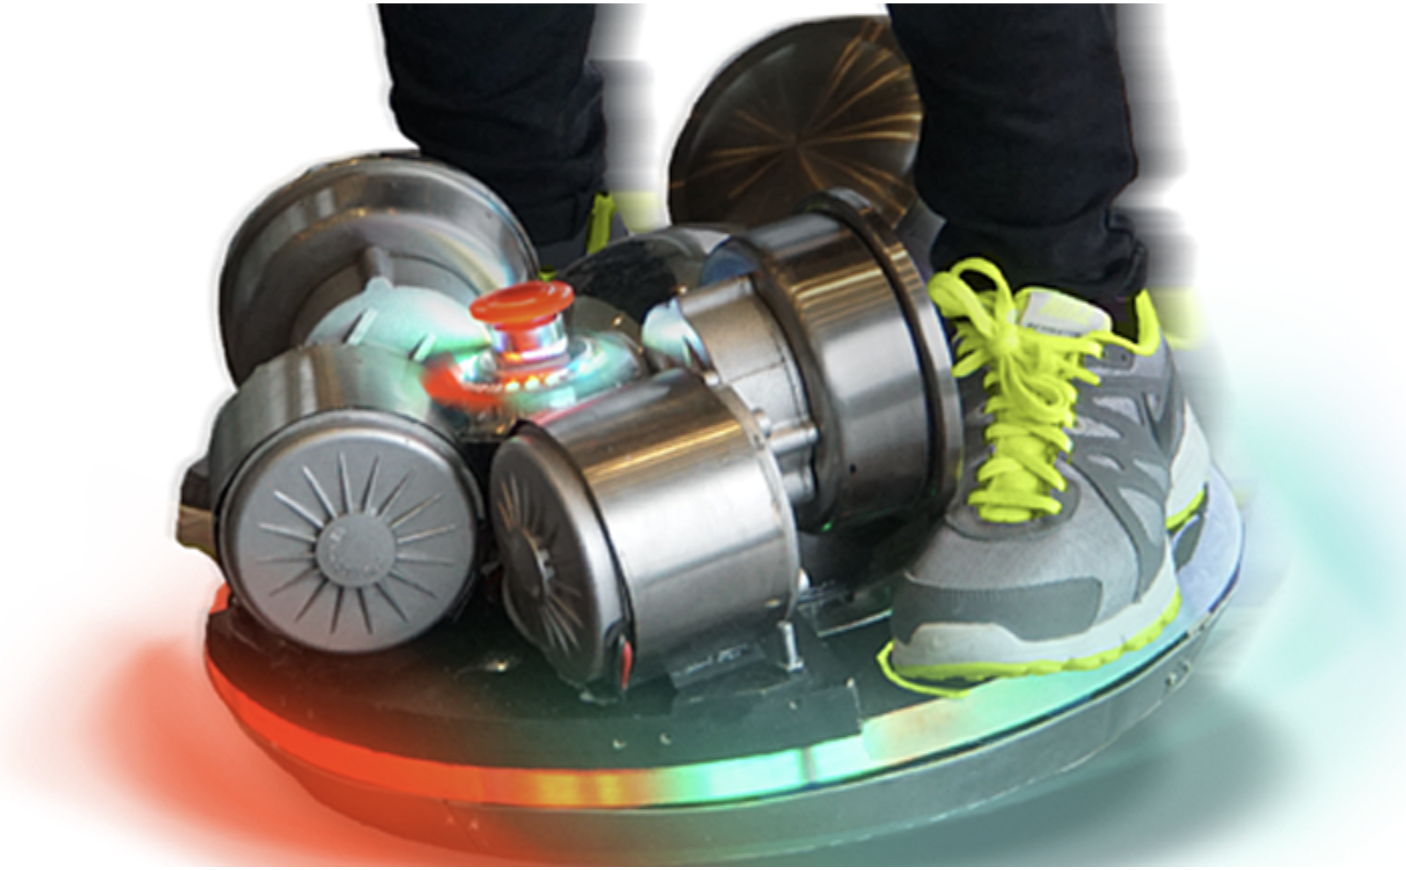
\includegraphics[height=0.25\textheight]{pdpAssets/SegwayStyleSelfBalancingPlatform.png} \\
\textbf{1. Ball Drive} & \textbf{2. Segway-Style} \\[0.15cm]
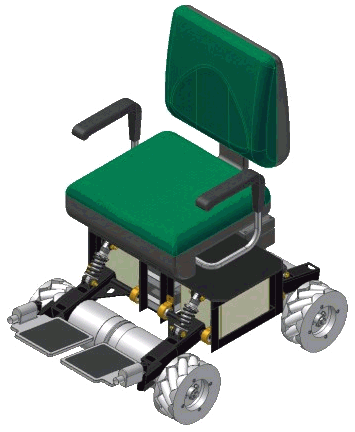
\includegraphics[height=0.25\textheight]{pdpAssets/MecanumWheelSystem.png} &
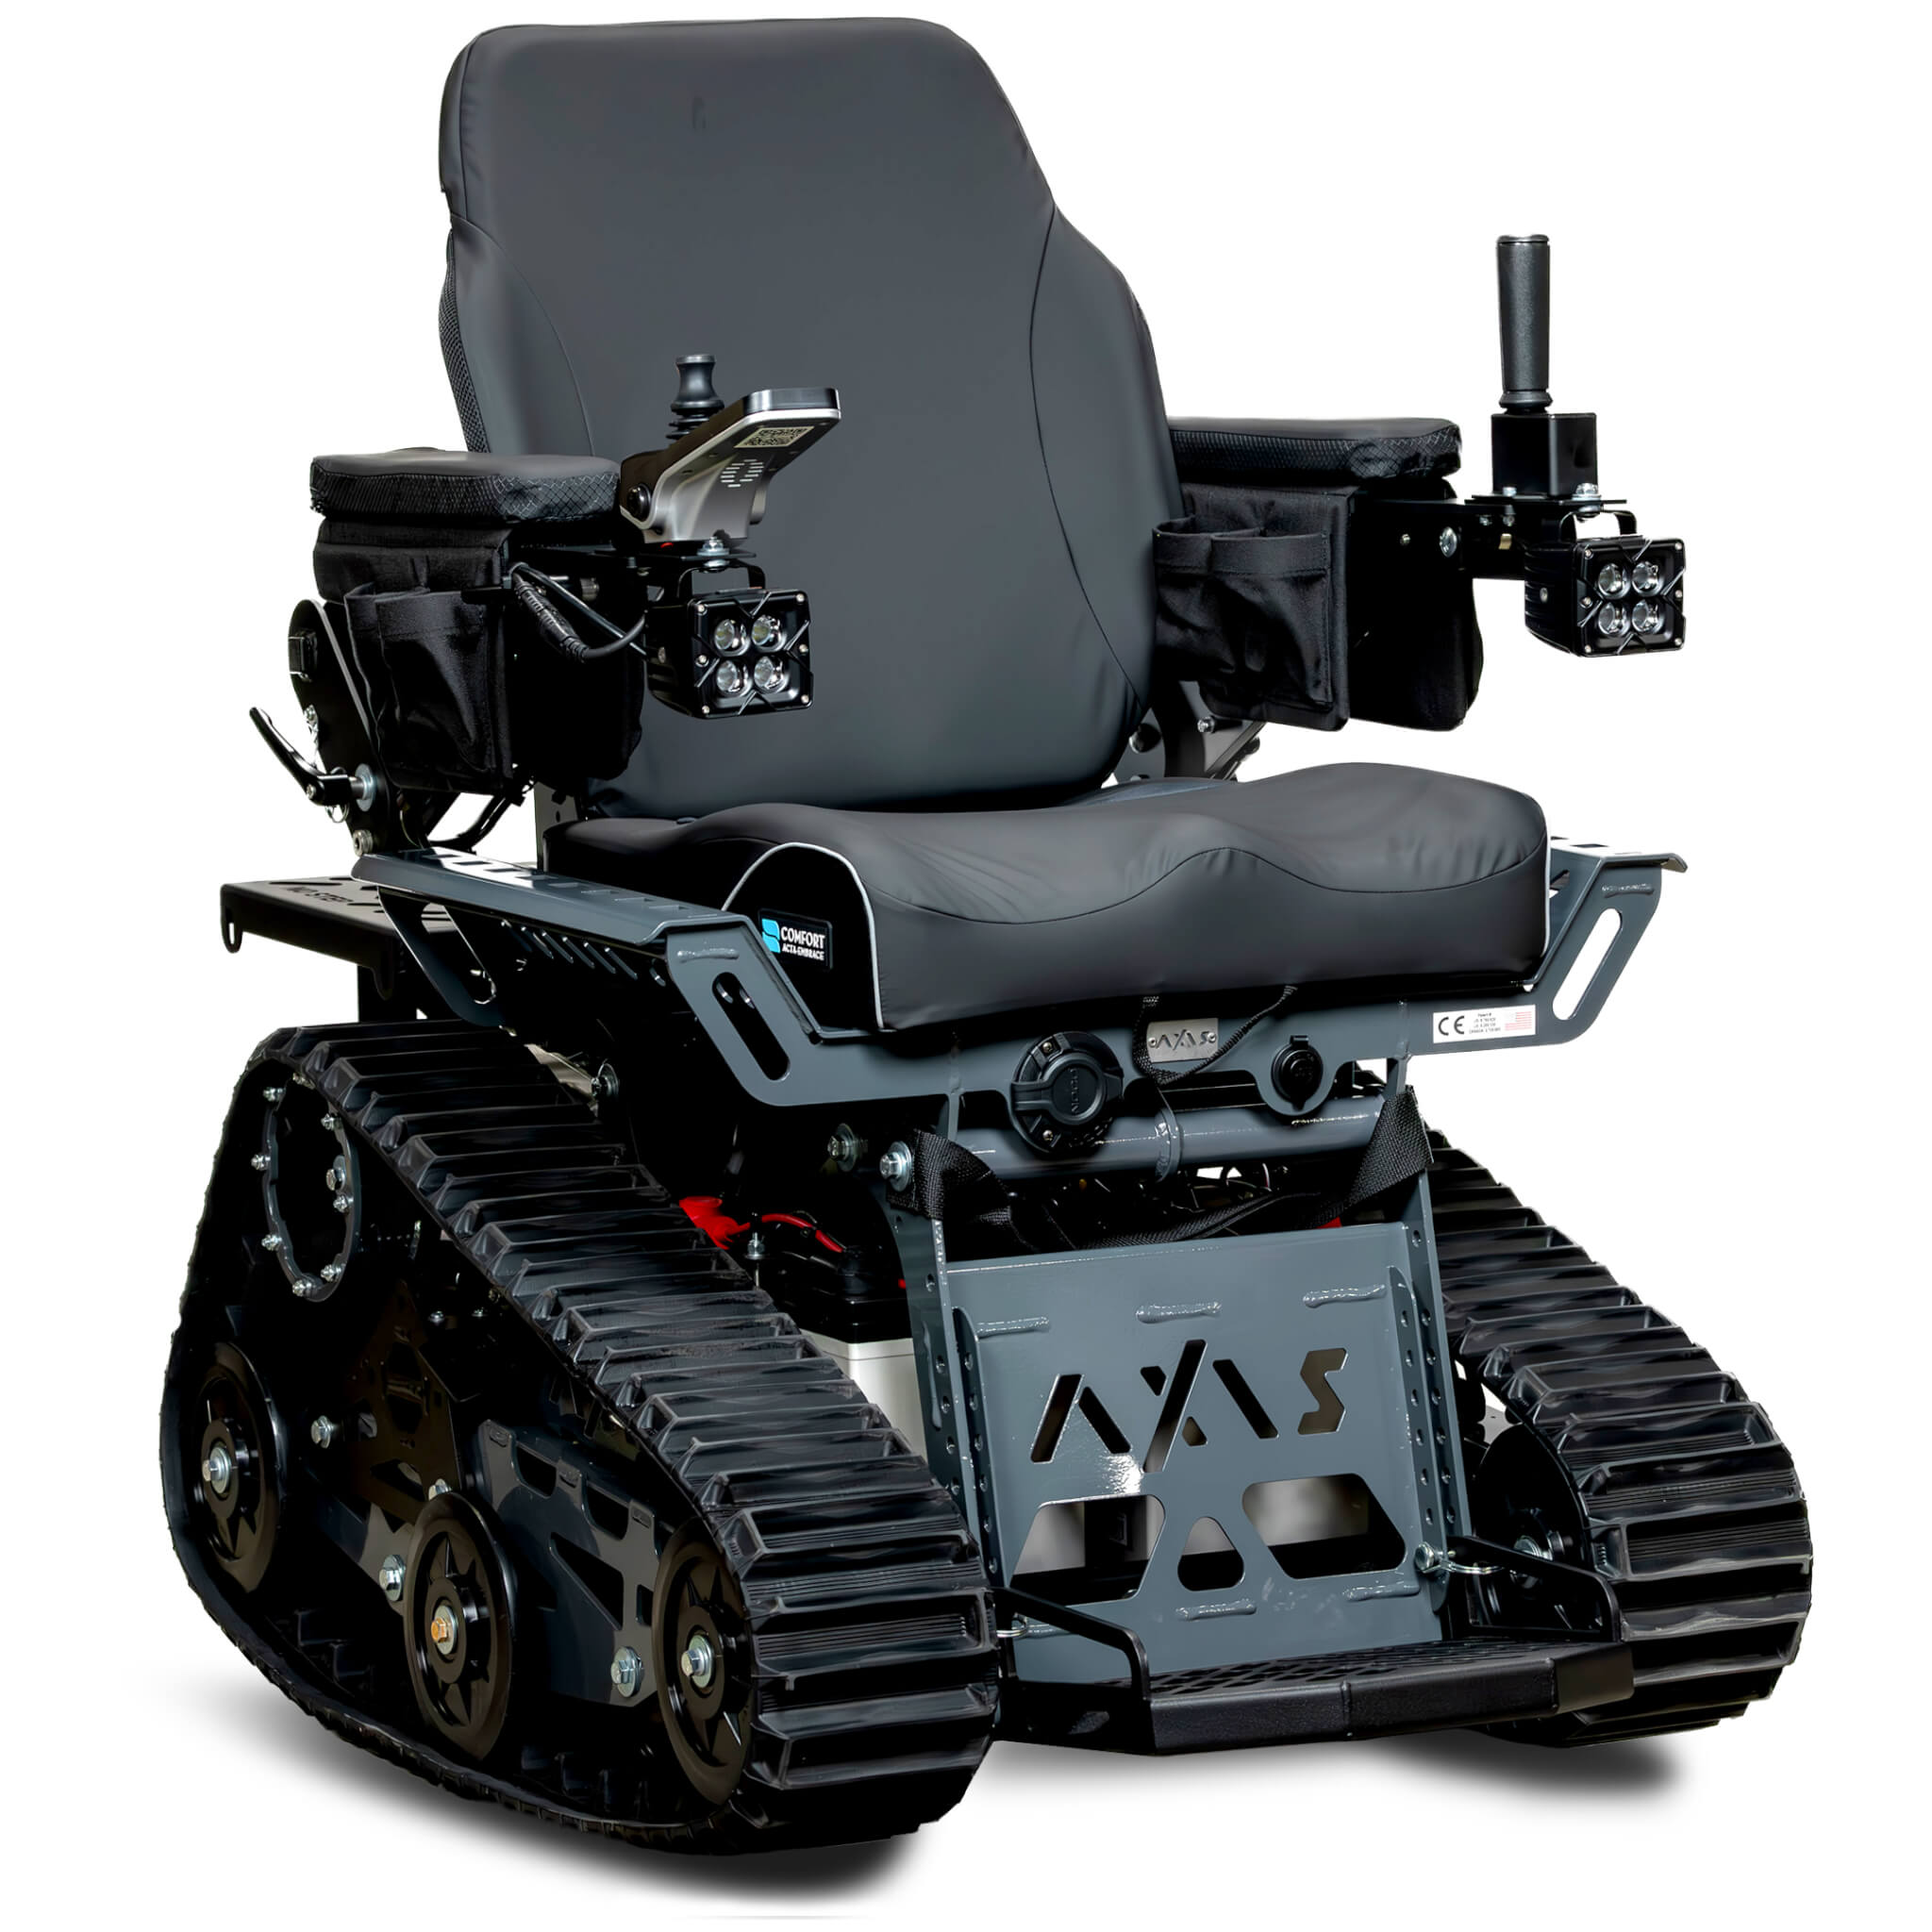
\includegraphics[height=0.25\textheight]{pdpAssets/TrackBasedSystemwithPivotMechanism.jpg} \\
\textbf{3. Mecanum Wheels} & \textbf{4. Track System} \\
\end{tabular}
\end{center}
\end{frame}

\begin{frame}{Design 1: Ball Drive System}
\begin{columns}[c]
\begin{column}{0.5\textwidth}
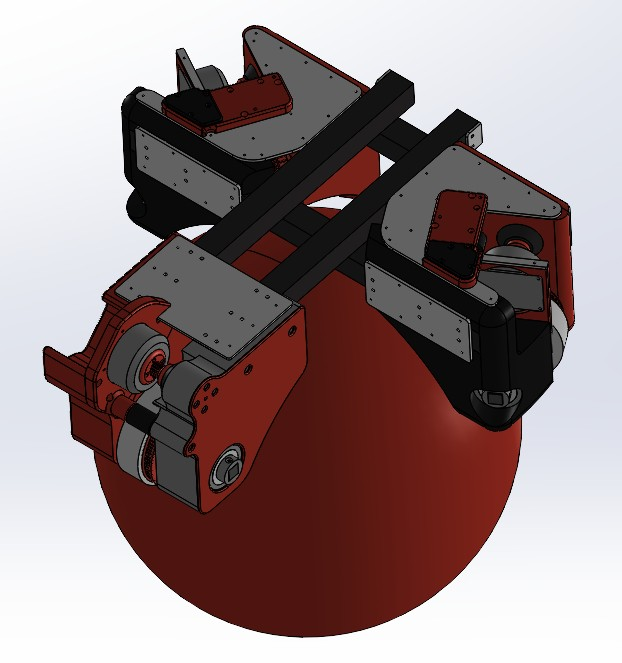
\includegraphics[height=0.6\textheight]{pdpAssets/PreliminaryDesignCadRendering.jpg}
\end{column}

\begin{column}{0.48\textwidth}
\begin{block}{Strengths}
\begin{itemize}
    \item True 360° movement
    \item Intuitive control
    \item Minimal protrusions
    \item Equipment compatible
\end{itemize}
\end{block}

\begin{block}{Weaknesses}
\begin{itemize}
    \item Complex mechanics
    \item Higher cost
    \item Maintenance needs
\end{itemize}
\end{block}
\end{column}
\end{columns}
\end{frame}

\begin{frame}{Design 2: Segway-Style Platform}
\begin{columns}[c]
\begin{column}{0.5\textwidth}
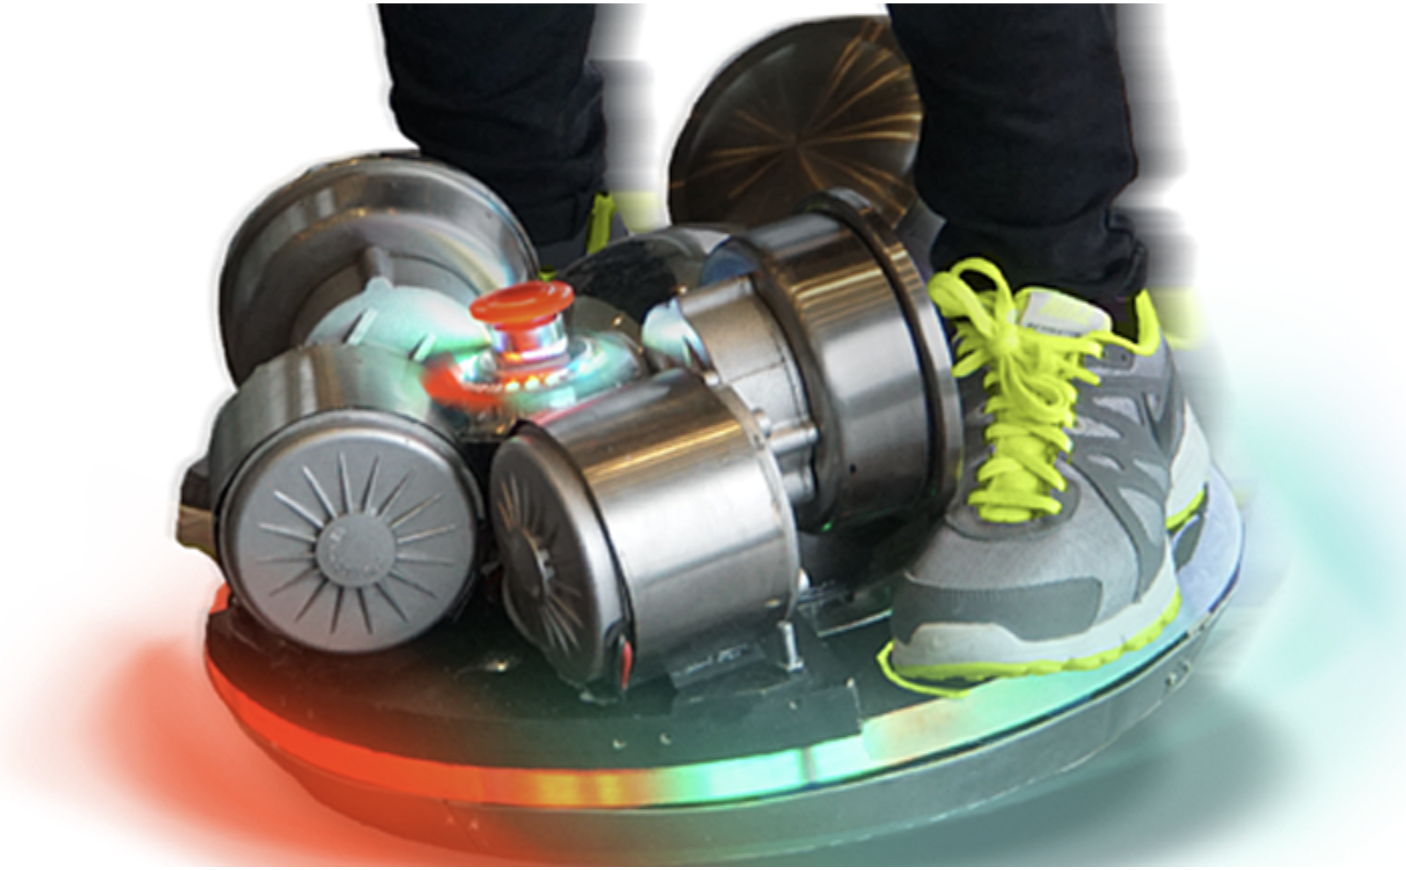
\includegraphics[height=0.6\textheight]{pdpAssets/SegwayStyleSelfBalancingPlatform.png}
\end{column}

\begin{column}{0.48\textwidth}
\begin{block}{Strengths}
\begin{itemize}
    \item Proven technology
    \item Excellent stability
    \item Responsive control
    \item Established manufacturing
\end{itemize}
\end{block}

\begin{block}{Weaknesses}
\begin{itemize}
    \item Only 2 DOF
    \item Poor sports compatibility
    \item Complex electronics
\end{itemize}
\end{block}
\end{column}
\end{columns}
\end{frame}

\begin{frame}{Design 3: Mecanum Wheels}
\begin{columns}[c]
\begin{column}{0.5\textwidth}
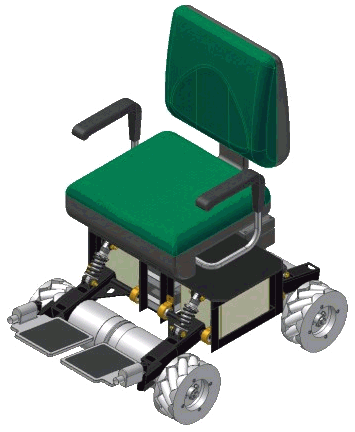
\includegraphics[height=0.6\textheight]{pdpAssets/MecanumWheelSystem.png}
\end{column}

\begin{column}{0.48\textwidth}
\begin{block}{Strengths}
\begin{itemize}
    \item Precise control
    \item Proven in robotics
    \item Good load distribution
    \item Modular design
\end{itemize}
\end{block}

\begin{block}{Weaknesses}
\begin{itemize}
    \item Complex wheels
    \item High maintenance
    \item Smooth surfaces only
    \item High cost
\end{itemize}
\end{block}
\end{column}
\end{columns}
\end{frame}

\begin{frame}{Design 4: Track System}
\begin{columns}[c]
\begin{column}{0.5\textwidth}
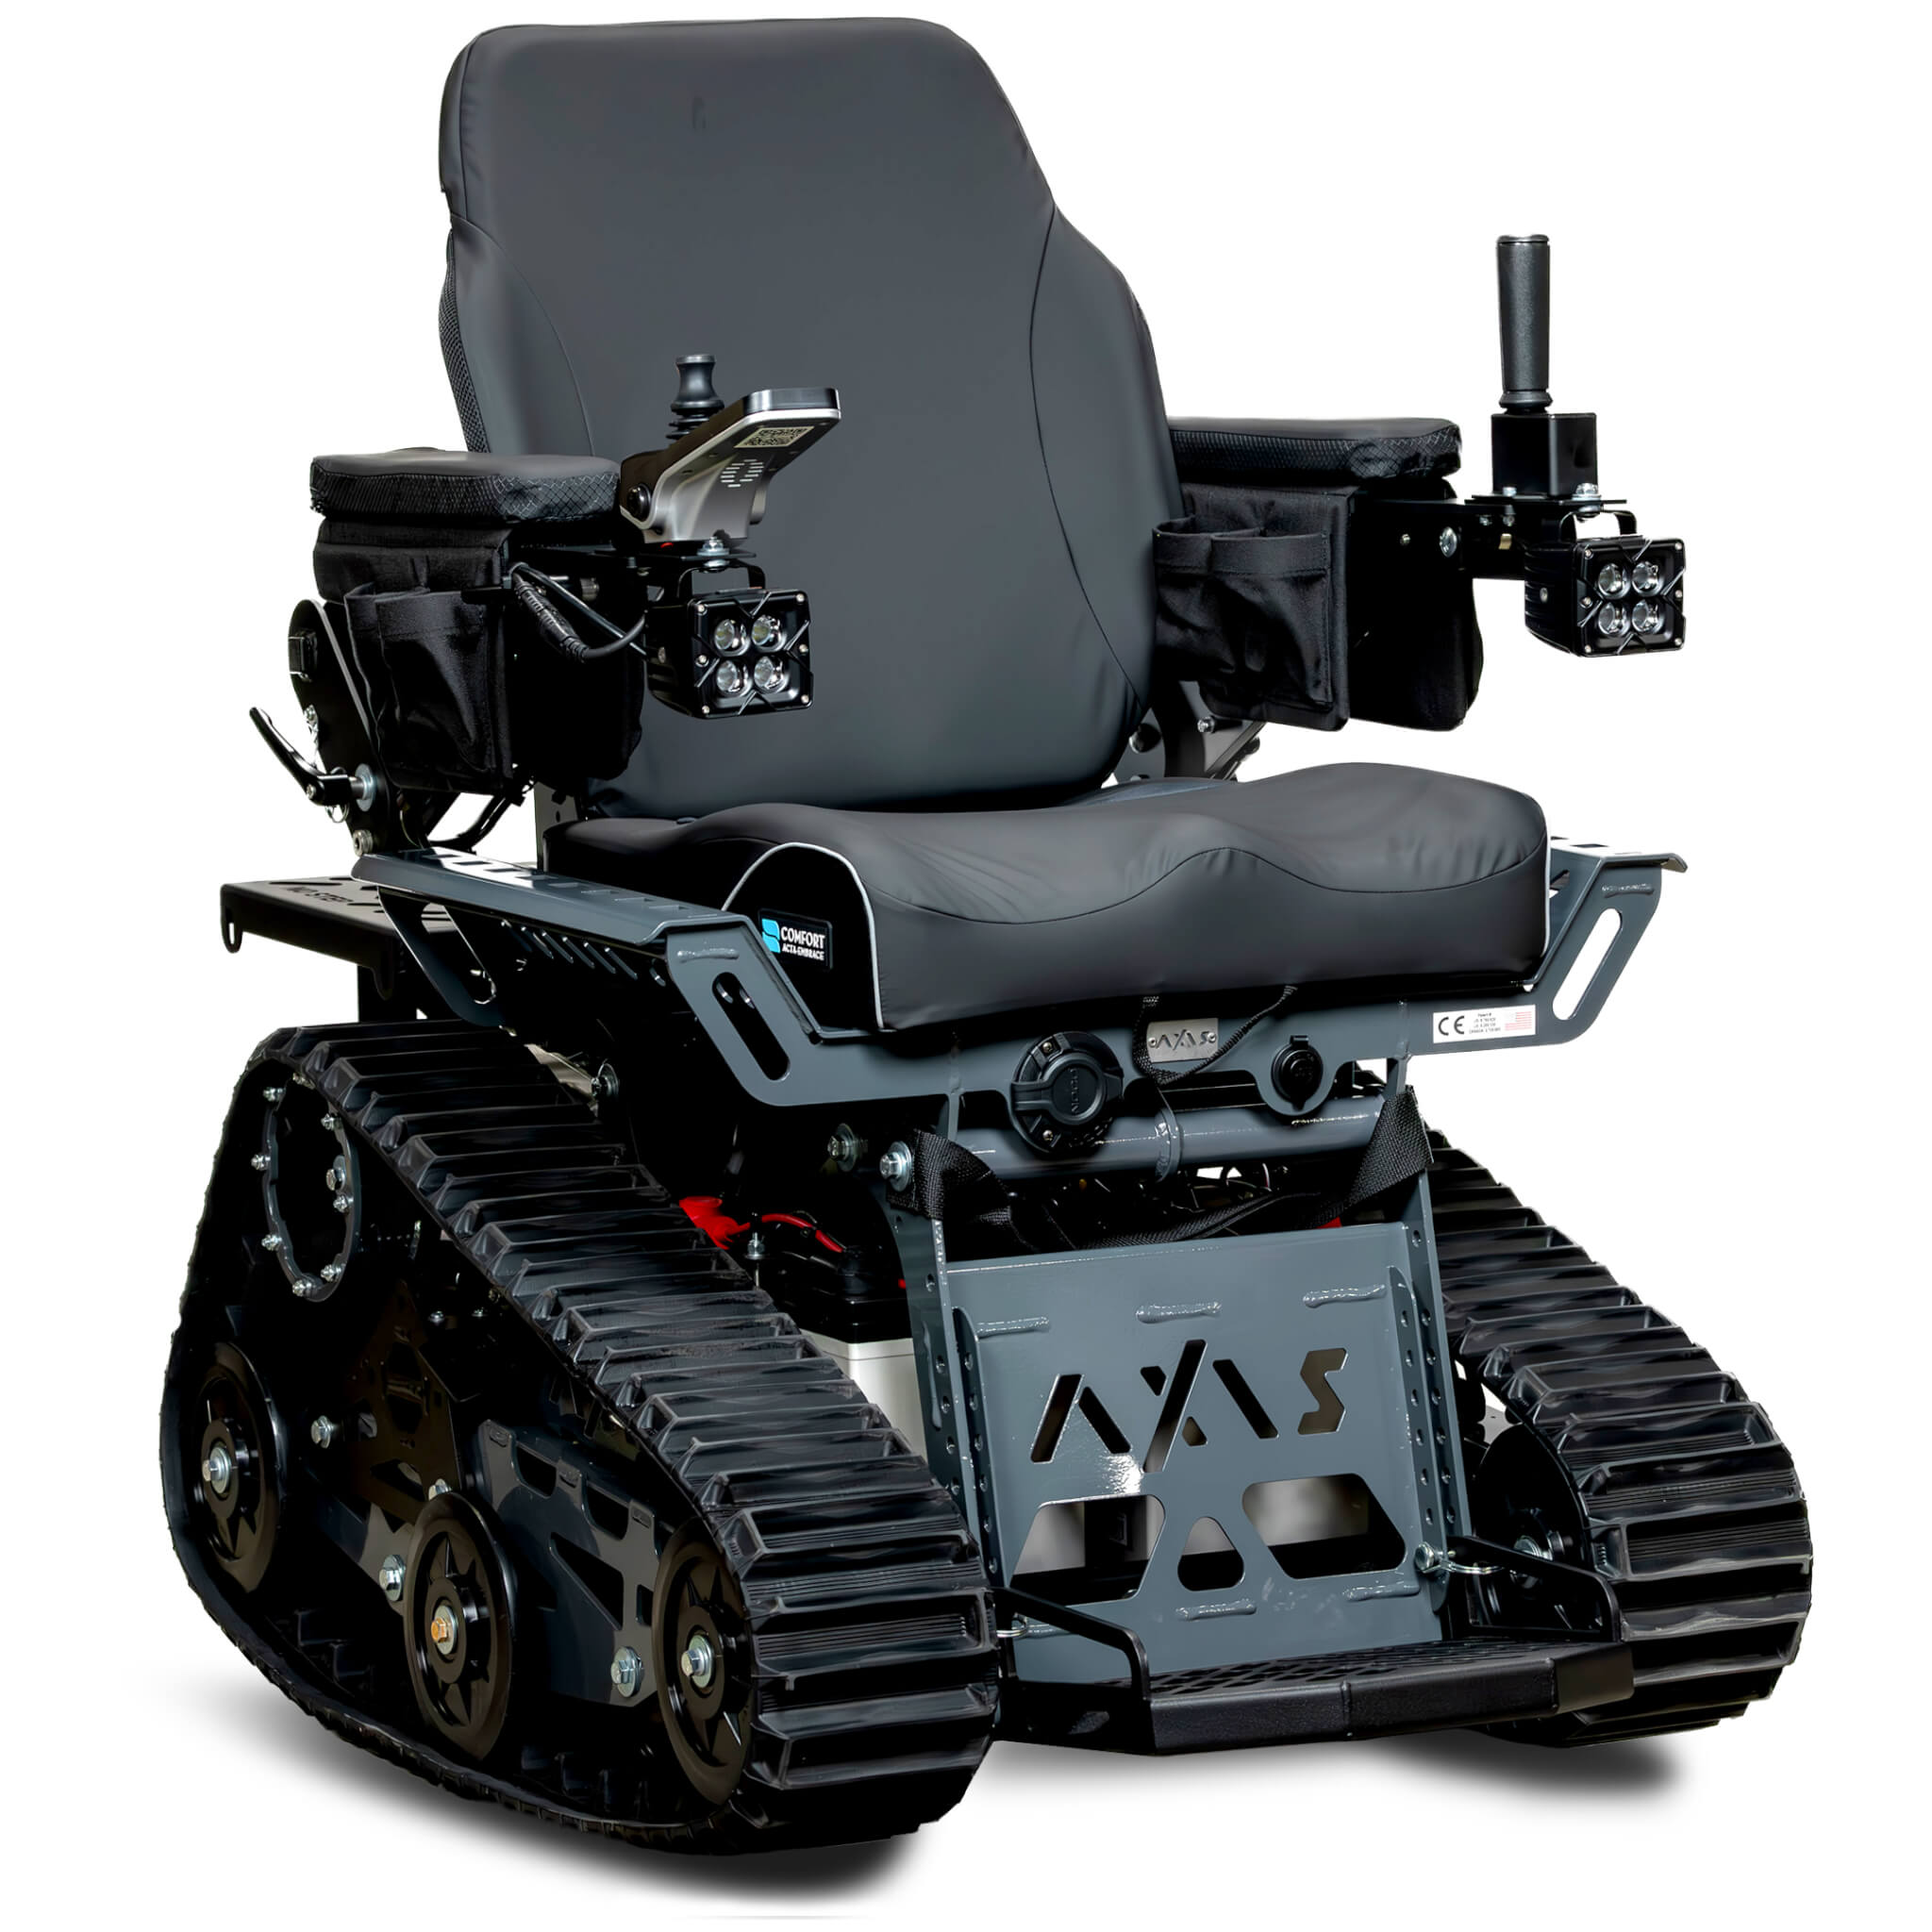
\includegraphics[height=0.6\textheight]{pdpAssets/TrackBasedSystemwithPivotMechanism.jpg}
\end{column}

\begin{column}{0.48\textwidth}
\begin{block}{Strengths}
\begin{itemize}
    \item Excellent traction
    \item Simple control
    \item Robust design
    \item Low maintenance
\end{itemize}
\end{block}

\begin{block}{Weaknesses}
\begin{itemize}
    \item Only 2 DOF
    \item Limited turning
    \item High friction
    \item Poor surface compatibility
\end{itemize}
\end{block}
\end{column}
\end{columns}
\end{frame}

\begin{frame}{Design Selection Matrix}
\footnotesize
\begin{table}
\centering
\begin{tabular}{lcccc}
\toprule
\textbf{Criteria (Weight)} & \textbf{Ball} & \textbf{Segway} & \textbf{Mecanum} & \textbf{Track} \\
\midrule
Hands-Free (25\%) & 9 & 8 & 9 & 7 \\
Non-Interfering (20\%) & 9 & 8 & 8 & 7 \\
Responsive (20\%) & 9 & 7 & 9 & 6 \\
Equipment Compat. (15\%) & 8 & 9 & 7 & 8 \\
Safety (10\%) & 7 & 9 & 8 & 9 \\
Intuitive (5\%) & 9 & 8 & 7 & 8 \\
Full Mobility (5\%) & 10 & 6 & 10 & 6 \\
\midrule
\textbf{WEIGHTED SCORE} & \textbf{8.6} & \textbf{7.7} & \textbf{8.3} & \textbf{7.1} \\
\bottomrule
\end{tabular}
\end{table}

\vspace{0.3cm}
\begin{center}
\Large \textcolor{darkblue}{\textbf{Selected: Ball Drive System (8.6/10)}}
\end{center}
\end{frame}

\begin{frame}{Our Selected Design}
\begin{center}
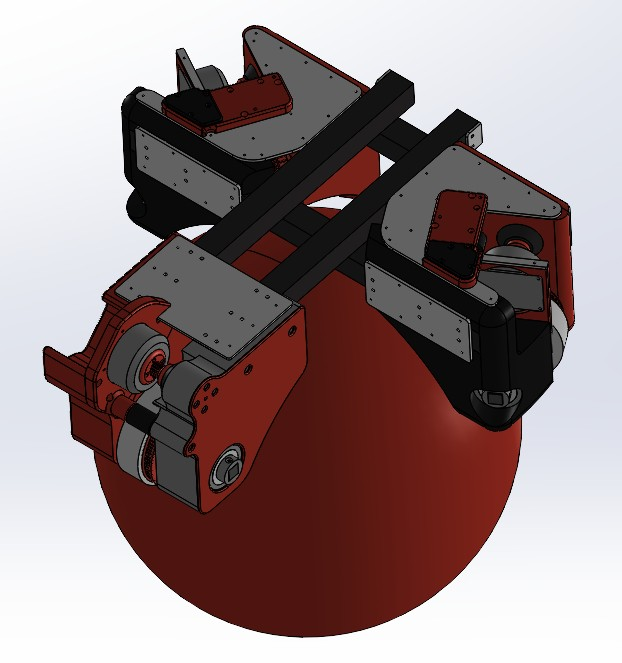
\includegraphics[height=0.7\textheight]{pdpAssets/PreliminaryDesignCadRendering.jpg}

\Large \textbf{Omni-Directional Ball Drive System}\\
\normalsize Score: 8.6/10
\end{center}
\end{frame}

%% SECTION 4: PATENT REVIEW
\section{Patent Review}

\begin{frame}{Patent Landscape}
\begin{center}
\begin{tabular}{ccc}
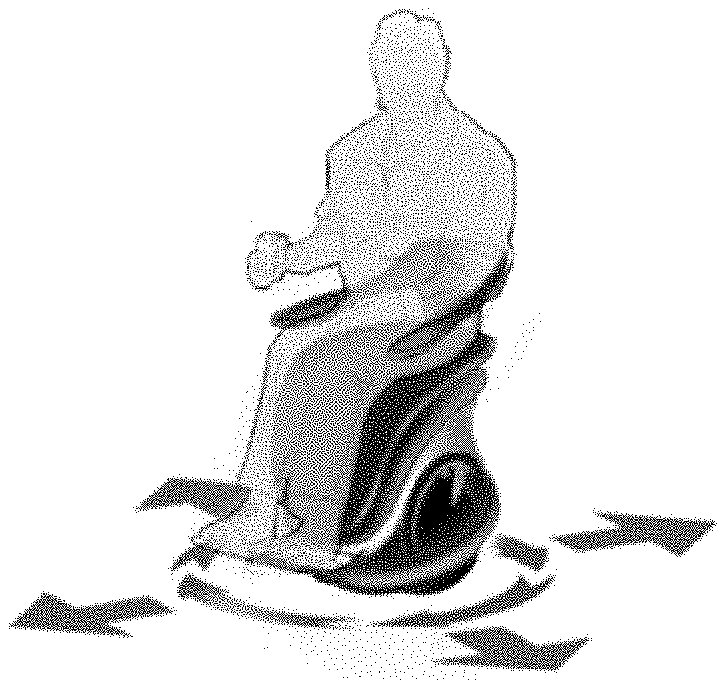
\includegraphics[width=0.28\textwidth]{pdpAssets/US20220062075A1.png} &
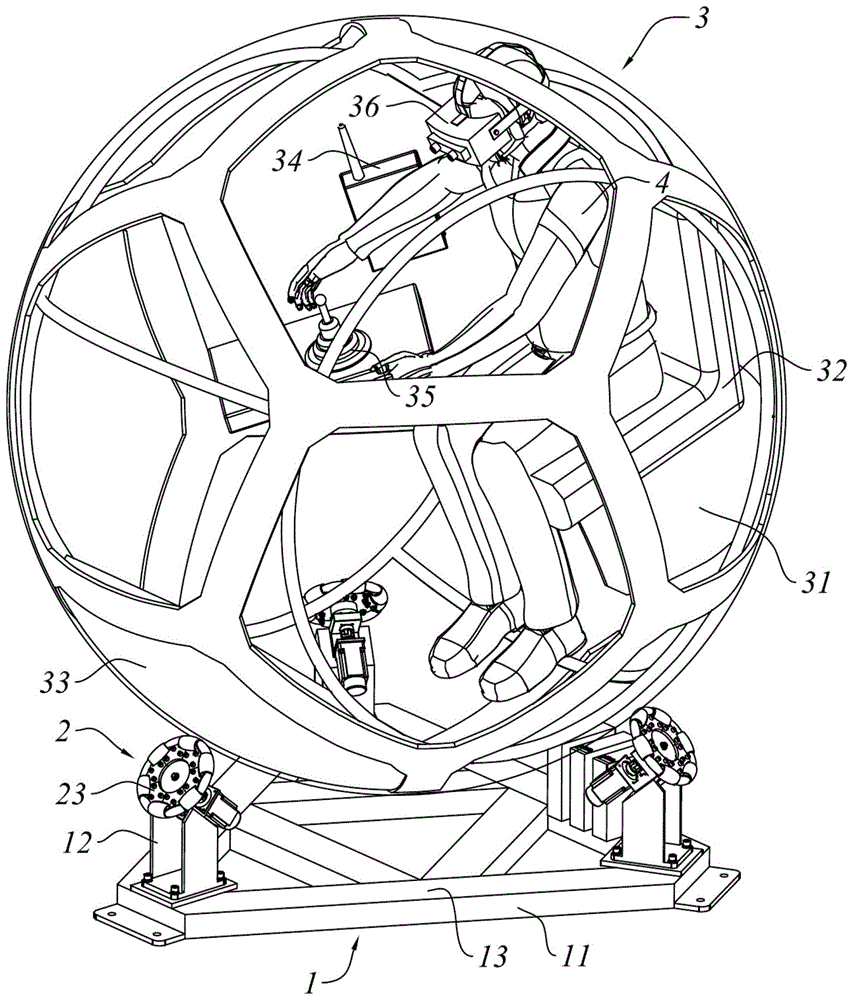
\includegraphics[width=0.28\textwidth]{pdpAssets/CN112071160A.png} &
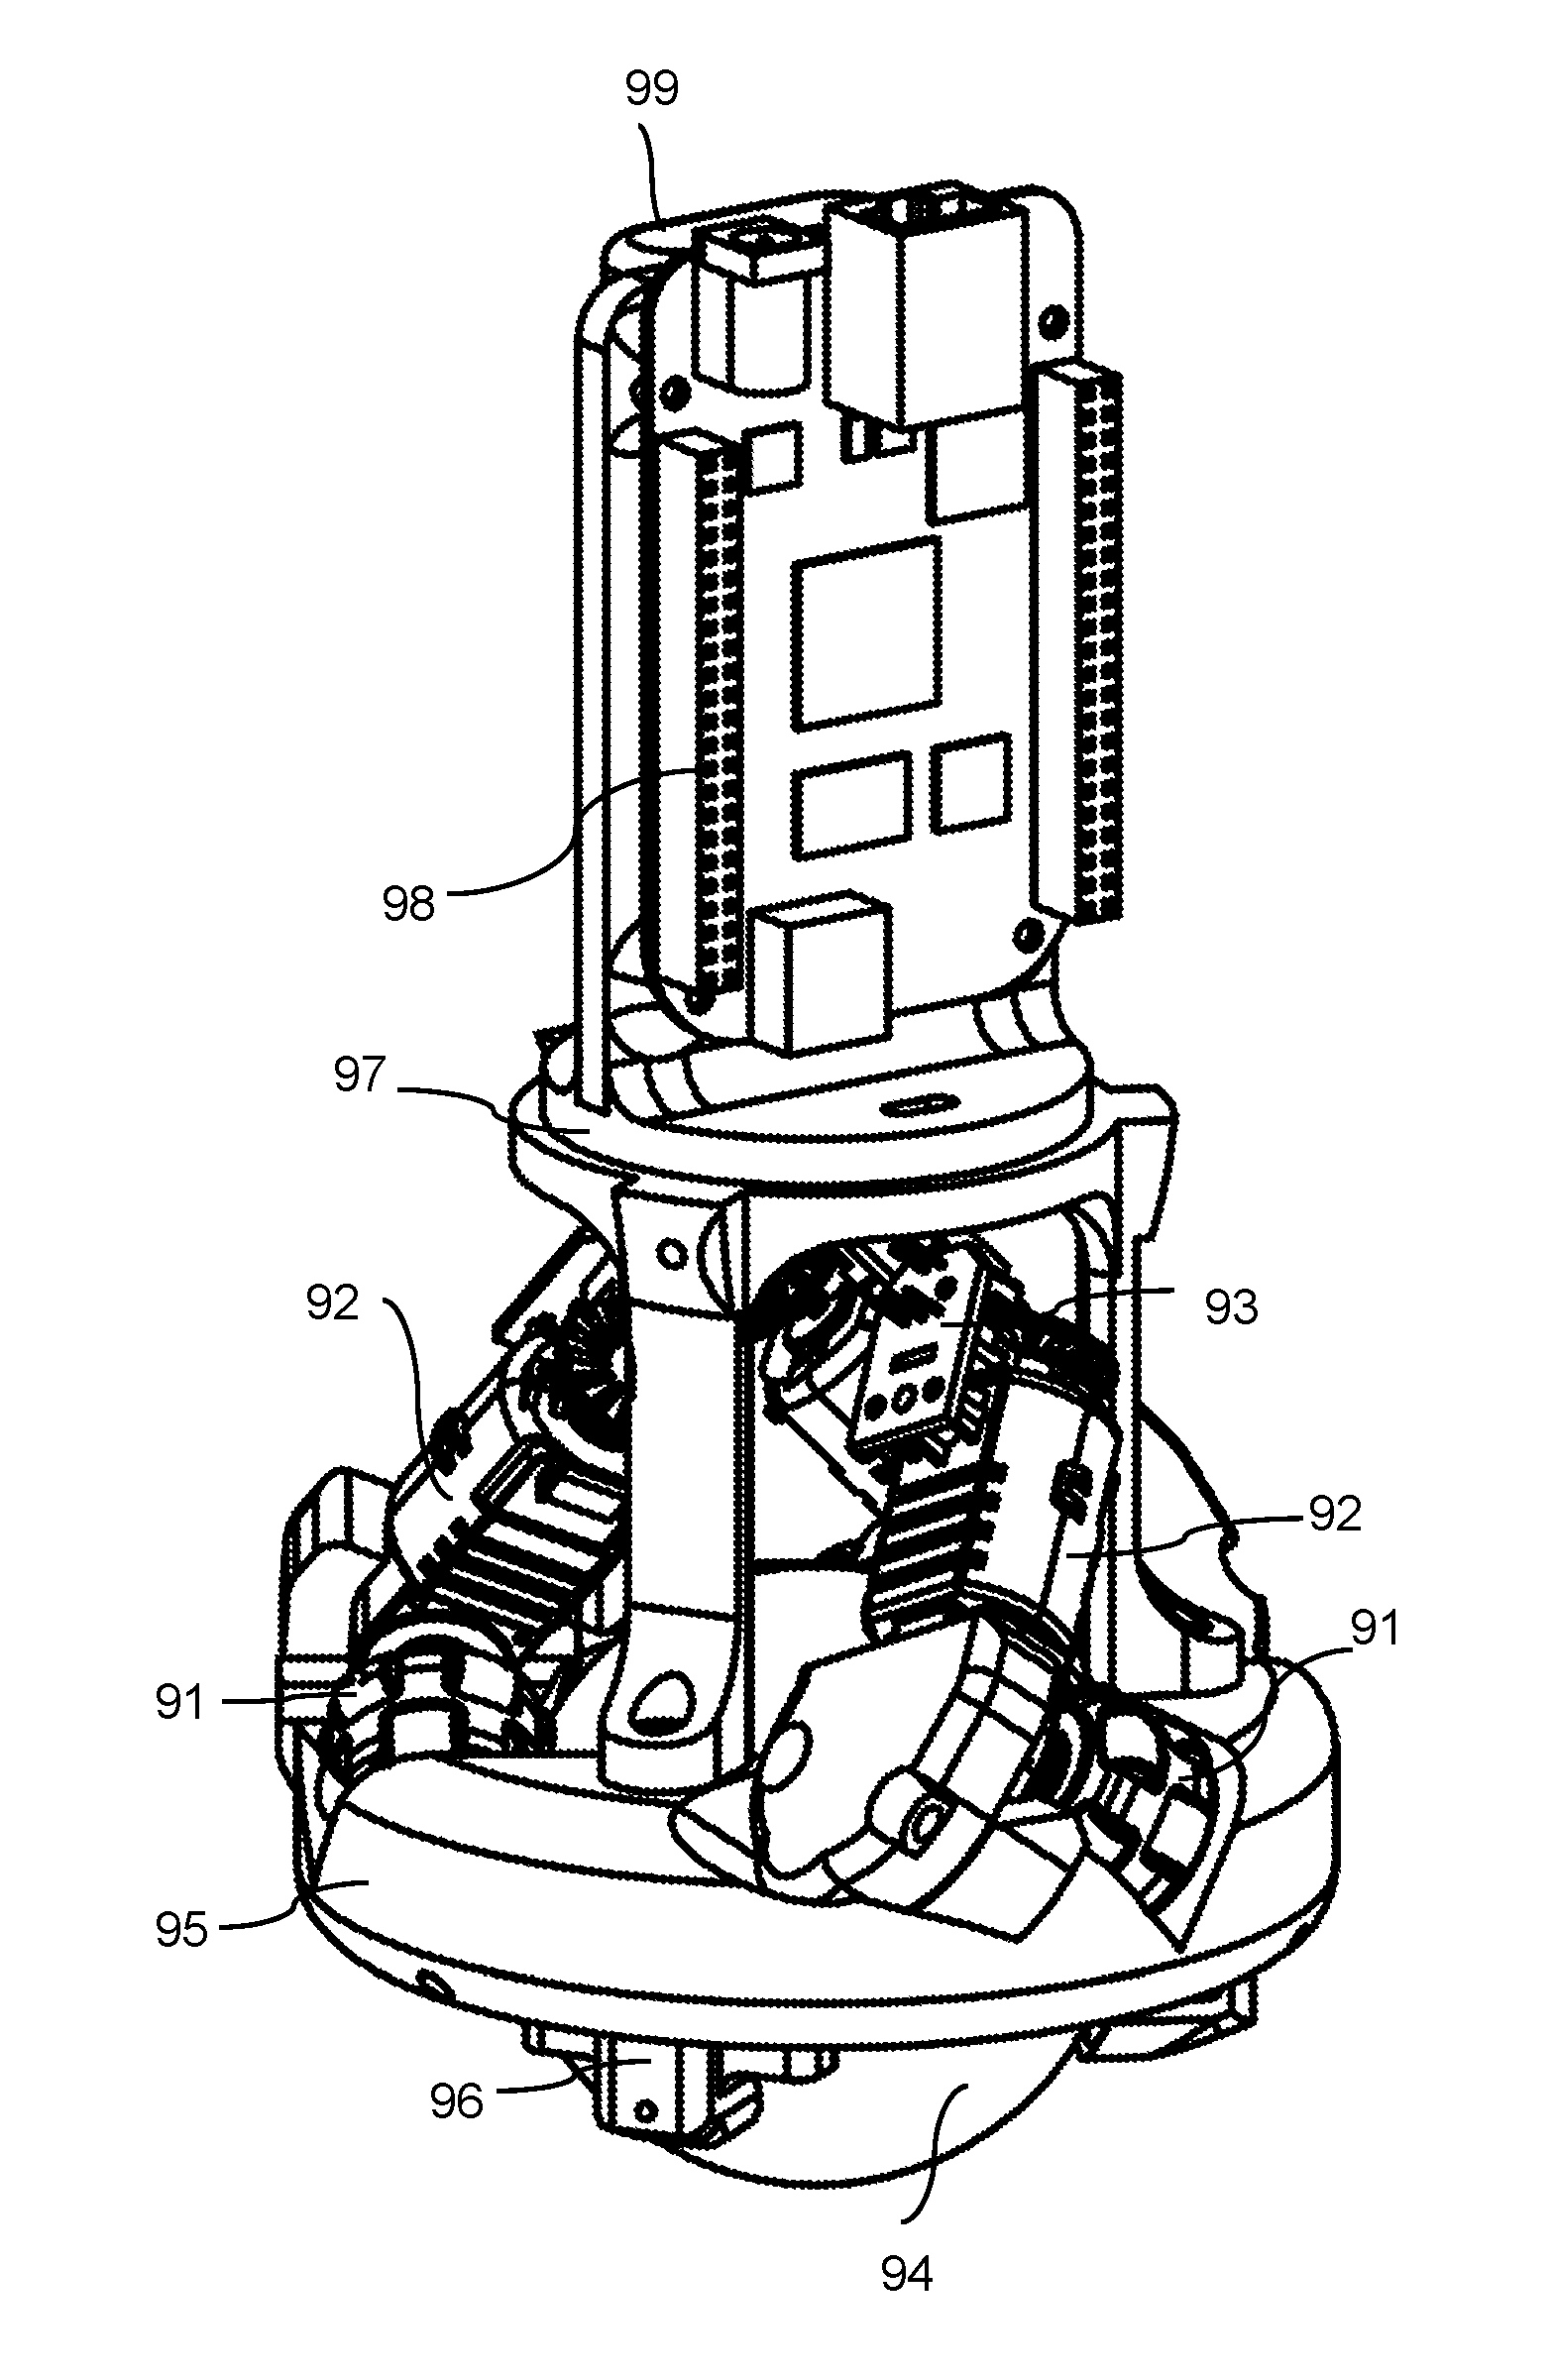
\includegraphics[width=0.28\textwidth]{pdpAssets/US20180022197A1.png} \\
\footnotesize US20220062075A1 & \footnotesize CN112071160A & \footnotesize US20180022197A1 \\
\footnotesize Omni-Dir Ball & \footnotesize Single Wheel & \footnotesize Multi-Dir Device \\
\end{tabular}
\end{center}

\vspace{0.3cm}
\begin{block}{Our Differentiation}
\begin{itemize}
    \item Multi-point contact (vs single wheel)
    \item Sports-specific optimization
    \item Enhanced collision resistance
    \item Equipment compatibility focus
\end{itemize}
\end{block}
\end{frame}

\begin{frame}{Design Freedom}
\begin{center}
\LARGE \textbf{Clear Path Forward}

\vspace{0.5cm}
\Large
Our innovation:
\end{center}

\begin{block}{Key Differentiators}
\begin{itemize}
    \item Multi-point ball contact system
    \item Sports-specific features
    \item Equipment compatibility focus
    \item Modular architecture
    \item Enhanced collision resistance
\end{itemize}
\end{block}

\vspace{0.5cm}
\begin{center}
\Large \textcolor{darkblue}{\textbf{Assessment: Clear Path Forward}}
\end{center}
\end{frame}

%% SECTION 5: TECHNICAL DETAILS
\section{Technical Details}

\begin{frame}{System Architecture}
\begin{columns}[T]
\begin{column}{0.48\textwidth}
\begin{block}{Control System}
\begin{itemize}
    \item Arduino Mega 2560
    \item \textbf{BNO085 IMU} (9-axis)
    \item \textbf{VESC-6 Controllers} (x2)
    \item I2C/SPI interfaces
\end{itemize}
\end{block}

\begin{block}{Mechanical}
\begin{itemize}
    \item 8" Ball Drive (2-drive layout)
    \item Aluminum Frame
    \item \textbf{BLDC Motors} (149 KV)
    \item 3:1 gear reduction
\end{itemize}
\end{block}
\end{column}

\begin{column}{0.48\textwidth}
\begin{block}{Power \& Safety}
\begin{itemize}
    \item \textbf{10S2P Li-ion} (36V, 6Ah)
    \item 216 Wh capacity
    \item Current limits: 25A cont, 60A peak
    \item Emergency stop
    \item Torque ramping
\end{itemize}
\end{block}

\vspace{0.3cm}
\begin{block}{Performance}
\begin{itemize}
    \item \textbf{5 N$\cdot$m torque} per motor
    \item \textbf{100W average} power
    \item Max speed: 1 m/s
    \item Real-time balance control
\end{itemize}
\end{block}
\end{column}
\end{columns}
\end{frame}

\begin{frame}{Key Performance Metrics}
\begin{center}
\Large \textbf{Engineering Specifications Summary}

\vspace{0.3cm}
\large
\begin{tabular}{ll}
\toprule
\textbf{Parameter} & \textbf{Target} \\
\midrule
Maximum Speed & 1 m/s (2.2 mph) \\
Response Time & $<100$ms \\
Battery Life & $>2$ hours (216 Wh) \\
Load Capacity & 80 kg (176 lbs) \\
Motor Torque & 5 N$\cdot$m per motor \\
Motor Power & 100W average \\
Degrees of Freedom & 3 DOF (omni-dir) \\
Tipping Resistance & 40N \\
Operating Temperature & 0-40°C \\
\bottomrule
\end{tabular}

\vspace{0.3cm}
\normalsize
\textit{Quantified targets based on user needs and engineering analysis}
\end{center}
\end{frame}

%% SECTION 6: TIMELINE
\section{Project Timeline}


\begin{frame}{Project Timeline}
\begin{center}
\Large \textbf{8-Month Development Schedule}

\vspace{0.5cm}
\footnotesize
\begin{tabular}{lcccccccc}
\toprule
\textbf{Phase/Activity} & \textbf{Sep} & \textbf{Oct} & \textbf{Nov} & \textbf{Dec} & \textbf{Jan} & \textbf{Feb} & \textbf{Mar} & \textbf{Apr} \\
\midrule
Idea Generation & \rule{1cm}{0.3cm} & & & & & & & \\
Preliminary Design & & \rule{0.8cm}{0.3cm} & & & & & & \\
\textcolor{red}{\textbf{PDP Presentation}} & & \textbf{$\bullet$} & & & & & & \\
Design Refinement & & & \rule{0.8cm}{0.3cm} & & & & & \\
Detailed Design & & & \rule{0.8cm}{0.3cm} & & & & & \\
Design Verification & & & & \rule{0.8cm}{0.3cm} & & & & \\
\textcolor{red}{\textbf{Final Presentation}} & & & & \textbf{$\bullet$} & & & & \\
Assembly \& Testing & & & & \rule{0.8cm}{0.3cm} & \rule{0.8cm}{0.3cm} & & & \\
Fabrication & & & & & \rule{0.8cm}{0.3cm} & \rule{0.8cm}{0.3cm} & & \\
Testing \& Optimization & & & & & & \rule{0.8cm}{0.3cm} & \rule{0.8cm}{0.3cm} & \\
Symposium Prep & & & & & & & \rule{0.8cm}{0.3cm} & \rule{0.8cm}{0.3cm} \\
\textcolor{red}{\textbf{Symposium}} & & & & & & & & \textbf{$\bullet$} \\
\bottomrule
\end{tabular}
\end{center}
\end{frame}

%% SUMMARY
\section{Summary}

\begin{frame}{Summary}
\begin{block}{Project Highlights}
\begin{itemize}
    \item Addresses critical need in wheelchair sports
    \item Research-backed problem identification (73\% injury rate)
    \item Comprehensive design evaluation (4 concepts)
    \item Clear technical specifications (30+ parameters)
    \item Within budget (\$230-320 vs \$300 limit)
    \item Feasible 8-month timeline
\end{itemize}
\end{block}

\vspace{0.3cm}
\begin{center}
\Large \textcolor{darkblue}{\textbf{Expected Impact: 25-40\% increase in wheelchair sports participation}}
\end{center}
\end{frame}

\begin{frame}[plain]
\begin{center}
\Huge \textbf{Thank you very much!}

\vspace{1cm}
\Large \textbf{Open for Questions!!}

\vspace{1.5cm}
\Large Capstone Group 52\\
MTE 481 - Fall 2025

\vspace{0.5cm}
\normalsize
Samuel | Ameen | Joseph | Chanuth | Adesh
\end{center}
\end{frame}

%% BACKUP SLIDES
\section*{Backup}

\begin{frame}{Detailed Specifications}
\tiny
\begin{tabular}{llll}
\toprule
\textbf{Category} & \textbf{Specification} & \textbf{Value} & \textbf{Justification} \\
\midrule
Mobility & Max Speed & 5 mph & Safe for indoor sports \\
& Acceleration & 0-5mph in 2s & Natural feel \\
& DOF & 3 DOF & Full mobility \\
Control & Response & <100ms & Real-time control \\
& IMU Rate & 100 Hz & Body tracking \\
Stability & CoG Height & <18 in & Tipping prevention \\
& Wheelbase & 24" x 24" & Stability polygon \\
Power & Battery & 7Ah @ 12V & 2+ hour runtime \\
& Motors & 25W each & Sufficient torque \\
\bottomrule
\end{tabular}
\end{frame}

\begin{frame}{Component Details}
\footnotesize
\begin{columns}[T]
\begin{column}{0.48\textwidth}
\begin{block}{Control System}
\begin{itemize}
    \item Arduino Mega 2560 (\$25-30)
    \item MPU-6050 IMU (\$5-8)
    \item L298N Driver (\$8-12)
\end{itemize}
\end{block}

\begin{block}{Mechanical}
\begin{itemize}
    \item 12V Motors x2 (\$15-20 ea)
    \item 8" Ball Mech (\$50-80)
    \item Al Frame (\$30-50)
\end{itemize}
\end{block}
\end{column}

\begin{column}{0.48\textwidth}
\begin{block}{Power \& Safety}
\begin{itemize}
    \item 12V 7Ah Battery (\$25-35)
    \item Protection Board (\$8-12)
    \item E-Stop Button (\$10-15)
    \item Speed Control (\$3-5)
\end{itemize}
\end{block}

\vspace{0.3cm}
\begin{block}{Total: \$230-320}
\end{block}
\end{column}
\end{columns}
\end{frame}

\begin{frame}{Constraints Analysis}
\footnotesize
\begin{itemize}
    \item \textbf{C1: Hands-Free} - 100\% movement without hand contact
    \item \textbf{C2: Safety} - 30-50N collision resistance, no tipping
    \item \textbf{C3: Equipment} - No interference with sports gear
    \item \textbf{C4: Environmental} - 5\% surface contamination tolerance
    \item \textbf{C5: Response} - <100ms sensor-to-motor lag
    \item \textbf{C6: Budget} - $<\$300$ total cost
    \item \textbf{C7: Timeline} - May 2026 deadline
\end{itemize}
\end{frame}

\end{document}